% Options for packages loaded elsewhere
\PassOptionsToPackage{unicode}{hyperref}
\PassOptionsToPackage{hyphens}{url}
%
\documentclass[
]{article}
\usepackage{amsmath,amssymb}
\usepackage{lmodern}
\usepackage{ifxetex,ifluatex}
\ifnum 0\ifxetex 1\fi\ifluatex 1\fi=0 % if pdftex
  \usepackage[T1]{fontenc}
  \usepackage[utf8]{inputenc}
  \usepackage{textcomp} % provide euro and other symbols
\else % if luatex or xetex
  \usepackage{unicode-math}
  \defaultfontfeatures{Scale=MatchLowercase}
  \defaultfontfeatures[\rmfamily]{Ligatures=TeX,Scale=1}
\fi
% Use upquote if available, for straight quotes in verbatim environments
\IfFileExists{upquote.sty}{\usepackage{upquote}}{}
\IfFileExists{microtype.sty}{% use microtype if available
  \usepackage[]{microtype}
  \UseMicrotypeSet[protrusion]{basicmath} % disable protrusion for tt fonts
}{}
\makeatletter
\@ifundefined{KOMAClassName}{% if non-KOMA class
  \IfFileExists{parskip.sty}{%
    \usepackage{parskip}
  }{% else
    \setlength{\parindent}{0pt}
    \setlength{\parskip}{6pt plus 2pt minus 1pt}}
}{% if KOMA class
  \KOMAoptions{parskip=half}}
\makeatother
\usepackage{xcolor}
\IfFileExists{xurl.sty}{\usepackage{xurl}}{} % add URL line breaks if available
\IfFileExists{bookmark.sty}{\usepackage{bookmark}}{\usepackage{hyperref}}
\hypersetup{
  pdfauthor={Aaron D. Lightner, Cynthiann Heckelsmiller, Edward H. Hagen},
  hidelinks,
  pdfcreator={LaTeX via pandoc}}
\urlstyle{same} % disable monospaced font for URLs
\usepackage[margin=1in]{geometry}
\usepackage{longtable,booktabs,array}
\usepackage{calc} % for calculating minipage widths
% Correct order of tables after \paragraph or \subparagraph
\usepackage{etoolbox}
\makeatletter
\patchcmd\longtable{\par}{\if@noskipsec\mbox{}\fi\par}{}{}
\makeatother
% Allow footnotes in longtable head/foot
\IfFileExists{footnotehyper.sty}{\usepackage{footnotehyper}}{\usepackage{footnote}}
\makesavenoteenv{longtable}
\usepackage{graphicx}
\makeatletter
\def\maxwidth{\ifdim\Gin@nat@width>\linewidth\linewidth\else\Gin@nat@width\fi}
\def\maxheight{\ifdim\Gin@nat@height>\textheight\textheight\else\Gin@nat@height\fi}
\makeatother
% Scale images if necessary, so that they will not overflow the page
% margins by default, and it is still possible to overwrite the defaults
% using explicit options in \includegraphics[width, height, ...]{}
\setkeys{Gin}{width=\maxwidth,height=\maxheight,keepaspectratio}
% Set default figure placement to htbp
\makeatletter
\def\fps@figure{htbp}
\makeatother
\setlength{\emergencystretch}{3em} % prevent overfull lines
\providecommand{\tightlist}{%
  \setlength{\itemsep}{0pt}\setlength{\parskip}{0pt}}
\setcounter{secnumdepth}{5}
\newcommand{\beginsupplement}{
  \setcounter{table}{0}  
  \renewcommand{\thetable}{S\arabic{table}} 
  \setcounter{figure}{0} 
  \renewcommand{\thefigure}{S\arabic{figure}}
}
\usepackage{tabularx}
\usepackage{booktabs}
\usepackage{booktabs}
\usepackage{longtable}
\usepackage{array}
\usepackage{multirow}
\usepackage{wrapfig}
\usepackage{float}
\usepackage{colortbl}
\usepackage{pdflscape}
\usepackage{tabu}
\usepackage{threeparttable}
\usepackage{threeparttablex}
\usepackage[normalem]{ulem}
\usepackage{makecell}
\usepackage{xcolor}
\ifluatex
  \usepackage{selnolig}  % disable illegal ligatures
\fi

\title{\LARGE \textbf{Supplementary Information for \emph{Ethnomedical specialists and their supernatural theories of disease}}}
\author{Aaron D. Lightner, Cynthiann Heckelsmiller, Edward H. Hagen}
\date{}

\begin{document}
\maketitle

{
\setcounter{tocdepth}{2}
\tableofcontents
}
\setcounter{table}{0}  
  \renewcommand{\thetable}{S\arabic{table}} 
  \setcounter{figure}{0} 
  \renewcommand{\thefigure}{S\arabic{figure}}

\hypertarget{supplementary-description-of-the-hypotheses-in-study-1}{%
\section{Supplementary description of the hypotheses in Study 1}\label{supplementary-description-of-the-hypotheses-in-study-1}}

In the main text we outlined and motivated four hypotheses, for which we tested the levels of support in the ethnographic record using the eHRAF. An absence of evidence does not constitute evidence of absence in the ethnographic record, but two hypotheses (\emph{efficacious healing} and \emph{prestigious mentors}) were amenable to opposing hypotheses, i.e., models that we could also find evidence for which stood in opposition to their counterparts (\emph{inefficacious healing} and \emph{low status}, respectively). These hypotheses, their descriptions, and the coded variables that supported them in this study are listed in table S1, and in figure 2 in the main text.

\hypertarget{additional-variable-groupings-in-study-1}{%
\subsection{Additional variable groupings in study 1}\label{additional-variable-groupings-in-study-1}}

Readers will notice that there are six hypotheses here, included in table S1 and figure 2 of the main text, but figure 2 contains a total of ten variable groupings. We should emphasize that there are additional variable groupings in figure 2 of the main text because they correspond not to the hypotheses in table S1, but to useful groupings that correspond to variables about client incentives vs.~disincentives for patronizing a specialist, and to variables about specialist knowledge attributes and social attributes. These are not hypotheses, but ways of dividing up the variables into useful and intuitive categories. See the main text for details.

\begin{table}[!ht]
    \centering
    \begin{tabularx}{\textwidth}{@{}lXX@{}}
        \toprule
        \textbf{Hypothesis}   & \textbf{Description}      & \textbf{Coded Variables}\\
        \midrule
        Religiosity  & 
          Ethnomedical specialists are religious figures and/or use supernatural theories of disease & 
          \begin{itemize}
          \item Supernatural
          \item Religious leadership
          \item Costly ritual
          \item Expert prescribes behavior/ritual
          \item Learns by revelation
          \end{itemize}  \\
        \hline
      Efficacious healing    & 
        Ethnomedical specialists employ techniques that are effective for diagnosing and/or treating illnesses that clients present to them  & 
        \begin{itemize}
          \item Evidence of success
          \item Reputation for efficacy
          \item Patronage based on efficacy
          \end{itemize}  \\
        \hline
        Inefficacious healing    & 
        Ethnomedical specialists employ techniques that are \emph{not} effective for diagnosing and/or treating illnesses that clients present to them  & 
        \begin{itemize}
          \item Evidence of failure
          \item Reputation for inefficacy
          \end{itemize}  \\
        \hline
        Market for specialists    & 
        Clients patronize ethnomedical specialists who confer benefits to them, with a preference or expectation for effective solutions to their problems, in a transactional exchange of services for payment  & 
        \begin{itemize}
          \item Payment to expert
          \item Knowledge distributed/multiple experts
          \item Narrow specialization
          \item Knowledge domain is not widespread
          \item Assists with uncommon/serious problem
          \end{itemize}  \\
        \hline
        Prestigious mentors    & 
        Acolytes seek proximity to prestigious ethnomedical specialists who teach in an apprenticeship or other (formal or informal) mentorship context  & 
        \begin{itemize}
          \item Prestige
          \item Trustworthy
          \item Others seek proximity to expert
          \item Reputation for generosity
          \item Expert teaches others
          \end{itemize}  \\
        \hline
        Low status    & 
        Ethnomedical specialists are in low status positions, are avoided and/or scorned by society, and are generally mistrusted  & 
        \begin{itemize}
          \item Anti-prestige/low status
          \item Not trustworthy
          \item Reputation for selfishness
          \item Others avoid the expert
          \end{itemize}  \\
        \hline
        \bottomrule
    \end{tabularx}
    \caption{\label{tab:vartable}Hypotheses and the coded variables that were tested in the cross-cultural ethnographic record in Study 1.}
\end{table}

\hypertarget{supplementary-descriptions-of-the-methods-in-study-1}{%
\section{Supplementary descriptions of the methods in Study 1}\label{supplementary-descriptions-of-the-methods-in-study-1}}

Here we provide details about the methods used for the results of the cross-cultural study in the main text, which was based on text records from the electronic Human Relations Area Files (eHRAF).

\hypertarget{statistical-analyses}{%
\subsection{Statistical analyses}\label{statistical-analyses}}

Our dataset, which comprised a 341 row by 58 column binary matrix of 0's (no evidence) and 1's (evidence for), consisted of text records (rows) nested within authors, who were nested within cultures. To assess levels of evidence for each variable, we determined the proportion of text records with evidence for (text record level evidence) and the proportion of cultures with at least one text record supporting the variable (culture level evidence). To account for the hierarchical structure of the data -- some text records came from the same document, and multiple documents reported on the same culture -- we fit an intercept-only generalized logistic mixed effects regression model (GLMM) for each binary variable, with random intercepts for authors nested within cultures. The value of the fixed-effect intercept (and its 95\% CI) represents the proportion of text records with evidence for a given variable, adjusted for the hierarchical structure of the data. The proportion of cultures with evidence for a given variable was similarly computed, except that its confidence interval was computed with cluster bootstrapping. We then converted each estimated proportion and its CI into percentages, which we reported as the variable's level of support.

To more formally assess and compare the levels of evidence for each hypothesized role of ethnomedical specialists (as efficacious healers, specialists in a market for useful skills, religious figures, and/or prestigious mentors), we grouped the variables relevant to each hypothesis and computed a ``total score'' for each. (We also include ``anti-efficacy'' and ``anti-mentorship'' hypotheses because some evidence against their counterparts was available.) The ``total score'' was the proportion of cells in the data matrix with evidence for each hypothesis. For example, our coding scheme included 6 religious variables, so there was a 341 \(\times\) 6 dimension binary matrix for this hypothesis. Of the 2046 cells, 459 (22.4\%) had evidence for religious variables. This percentage was the total score, and hypotheses with higher total scores were judged to have more support.

\hypertarget{exploratory-analyses-of-religiosity-and-the-supernatural}{%
\subsubsection{Exploratory analyses of religiosity and the supernatural}\label{exploratory-analyses-of-religiosity-and-the-supernatural}}

To explore religiosity (measured by the total score for religious variables) and the presence/absence of supernatural theories of disease, we used three key techniques.

First, to determine the dimensions of ethnomedical expertise that are associated with religiosity and the supernatural, we fit a poisson regression model with the text record religion scores as the outcome and a logistic regression model with text record supernatural theories (present/absent) as the outcome. In each model, the remaining coded variables on ethnomedical expertise were predictors. Prior to fitting, we removed variables with almost no evidence (\textgreater95\% zeros) to avoid spuriously large estimates and CI's. Because inclusion of many predictors risks overfitting, we used \emph{elasticnet} regression (Friedman 2021), a popular type of penalized regression that was developed for use in situations where the number of predictors, \(p\) is large relative to the number of observations, \(n\). We used the ``lasso'' penalty, which sets some coefficients to 0, with the non-zero coefficients representing the ``best'' predictors, given the limitations of the data. (See below for a brief description of the elasticnet regression.)

Second, to determine if continental region and/or mode of subsistence were associated with religiosity and the supernatural among ethnomedical specialists, we fit two separate logistic GLMMs with presence/absence of supernatural theories in each text record as the outcome variable. In one model, continental region of each of the 47 cultures was the predictor variable, and in the other model, subsistence strategy for each of these cultures was the predictor variable. In both models, we included random intercepts for cultures. We then repeated this process using two separate poisson GLMMs, with religion scores in each text record as the outcome variable.

Third, to determine if dimensions of cultures other than their continental region or mode of subsistence were associated with religiosity and supernatural theories of disease, we first compiled all complete quantitative data on 186 cultures from the Standard Cross Cultural Sample (SCCS) from D-PLACE (Kirby et al.~2016) into a dataset. Specifically, we collected all ordinal and continuous variables from the SCCS, and filtered all variables with missing observations. The resulting dataset contained 44 variables with observations for all 186 societies in the SCCS.

We then scaled the entire SCCS data matrix and conducted a principal components analysis (PCA) to reduce the dimensionality of the cross-cultural data. We retained the largest principal components based on variance explained (a scree plot ``elbow'') and interpretability, along with the principal component values for each culture that was also in our eHRAF dataset of ethnomedical specialists (the \emph{PCs}). Out of the 47 cultures in our eHRAF dataset, 44 cultures were also in the SCCS. We excluded the remaining 3 cultures from this analysis. In a logistic GLMM, we then modeled presence/absence of supernatural theories for each text record as the outcome, culture-level PCs as the predictors, and random intercepts for cultures.

\hypertarget{exploratory-analyses-of-markets-and-mentorship}{%
\subsubsection{Exploratory analyses of markets and mentorship}\label{exploratory-analyses-of-markets-and-mentorship}}

To explore the roles of market specialization, efficacy, and mentorship, we used two additional techniques.

First, at the text record level, we weighed the levels of evidence for common incentives for laypersons to patronize ethnomedical specialists (see figure 2 in the main text). In some cases, we also had evidence for corresponding disincentives (e.g., reputation for efficacy vs.~reputation for inefficacy); in other cases, we had evidence for contrasting incentives (e.g., assistance with uncommon and serious problems vs.~assistance common and everyday problems). To compare the weight of evidence for incentives vs.~disincentives, or for contrasting incentives, we used logistic regression to compute the odds ratios of evidence for one vs.~the other. Our comparisons were: \emph{specialists conferring benefits} vs.~imposing costs; \emph{reputations for efficacy} vs.~reputations for inefficacy; \emph{assistance with uncommon and serious problems} vs.~assistance common and everyday problems; \emph{patronage based on efficacy} vs.~patronage based on tradition, convenience, or cost (referred to as ``socioeconomic'' considerations); \emph{evidence of success} vs.~evidence of failure; \emph{trustworthy specialists} vs.~untrustworthy specialists; and \emph{freely shared services} vs.~services for payment.

Second, we assessed which variables were associated with an expansion of the market for ethnomedical specialists. As a proxy for presence/absence of expanding markets, we used the acculturation variable, which usually included presence/absence of foreign hospitals and clinics nearby and, in some cases, ethnomedical specialists from other cultures. Here, we modeled each of our coded variables as the outcome in separate logistic GLMMs, with the acculturation variable as the predictor (i.e., presence/absence of foreign hospitals and clinics nearby and, in some cases, ethnomedical specialists from other cultures) for each model, and authors nested within cultures as random intercepts.

\hypertarget{exploratory-analysis-of-the-variables-in-our-data}{%
\subsubsection{Exploratory analysis of the variables in our data}\label{exploratory-analysis-of-the-variables-in-our-data}}

Finally, to examine structure in our entire data matrix, i.e., to determine which groups of variables tended to have evidence in the same text records and therefore might indicate important abstractions about ethnomedical expertise, we used a network clustering technique known as a minimum spanning tree (MST). We computed the square matrix of all pairwise binary distances between column vectors in our dataset, where a binary distance = 0 means that two variables both had evidence in exactly the same text records, and a binary distance = 1 means that two variables never had evidence in the same text records. The resulting matrix can be conceptualized as an adjacency matrix that defines a weighted graph (\(G\)), where each vertex is a variable and each weighted edge is the distance between these variables.

From this we computed the MST, which is a subgraph of \(G\) in which every node is connected in a single path, minimizing the total weighted path distance without creating any closed paths (Prim 1957; Dijkstra 1959). In the resulting MST, only similar variables (the vertices) are connected to each other. We then identified ``clusters'' of variables by visual inspection of the MST, seeking groups of adjacent variables that were conceptually related.

\hypertarget{explanation-of-the-elasticnet-regression-model}{%
\subsection{Explanation of the elasticnet regression model}\label{explanation-of-the-elasticnet-regression-model}}

Here, we briefly describe the elasticnet regression model. Standard regression models are fit by minimizing an objective function. In ordinary least squares regression the objective function is the residual sum of squares (\(RSS\)), and in logistic regression it is the negative log-likelihood, \(-loglik(\beta)\). Penalized regression models instead minimizes the objective function plus a penalty term based on the magnitude of the coefficient vector. For linear regression this is:

\[
\frac{1}{2}RSS/n + \lambda * penalty
\]

and for logistic regression:

\[
-loglik(\beta)/n + \lambda * penalty
\]

\[
% l^{\lambda}(\beta) = l(\beta) - \lambda\sum_{j=1}^p\beta_j^2
\]

There are two popular forms of penalized regression: ridge regression and lasso regression. For ridge regression the penalty is \(||\beta||_2^2 = \sum_{j=1}^p\beta_j^2\), where the \(\beta_j\) are the regression coefficients, and for lasso regression the penalty is \(||\beta||_1 = \sum_{j=1}^p|\beta_j|\). When \(\lambda=0\), this reduces to the standard estimation. As \(\lambda \rightarrow \infty\), the coefficients \(\beta_j\) are ``shrunk'' to 0. Thus, when \(\lambda\) is small, the \(\beta s\) are relatively unrestricted, which can result in a good fit to the current sample (low bias), but a poor fit on future samples (high variance); roughly, the model will tend to be over-fitted. When \(\lambda\) is large, the \(\beta s\) tend to shrink toward 0, which reduces fit on the current sample (high bias), but results in a more stable fit across samples (low variance); roughly, the model will tend to be under-fitted. The optimal value of \(\lambda\) is typically found by minimizing cross-validation error.

With the lasso penalty, some coefficients might be set to 0, i.e., dropped from the model, which aids interpretation, but when variables are correlated, the lasso might drop some that are genuinely related to the outcome. In ridge regression, in contrast, the coefficients of correlated variables are shrunk to similar values; although the coefficients of some predictors might be very small, all predictors are retained in the model, which can make interpretation difficult.

Elastic net regression combines the advantages of ridge and lasso penalties using an additional tuning parameter \(\alpha\), \(0\leq \alpha \leq1\):

\[
penalty = (1-\alpha)/2||\beta||_2^2+\alpha||\beta||_1.
\]

Thus, \(\alpha=0\) is the ridge penalty and \(\alpha=1\) is the lasso penalty. With intermediate values of \(\alpha\), there is a `grouping' effect in which strongly correlated variables tend to enter or leave the model together (i.e., have their coefficients set to 0).

In the main text, we used elastic net regression to fit a logistic regression model of each domain type (conceptual, motor, medicine) as functions of our other coded (binary) variables. Following standard procedure, we used 10-fold cross-validation to find the optimum value of \(\lambda\), i.e., the one that minimized cross-validation error.

\hypertarget{description-of-our-search-query-in-the-ehraf}{%
\subsection{Description of our search query in the eHRAF}\label{description-of-our-search-query-in-the-ehraf}}

In the original Lightner et al.~(2021) study, we collected text records from the electronic Human Relations Area Files World Cultures database while intentionally targeting those that reflect some kind of ``{[}ethno{]}scientific expertise'' in the ethnographic literature. Inclusion was therefore based on descriptions of specialized expertise in a potentially relevant conceptual knowledge domains, such as botany, zoology, meteorology, genealogy, traditional history, conflict resolution, wartime strategies, illness, disease, life and death, and physiology. Our exact search query, i.e., the set of OCM codes and search terms that generated our initial results, was:

\begin{quote}
(( Cultures = (Any Culture ) ) AND ( ( ( Subjects = (`173' OR `278' OR `571' OR `577' OR `578' OR `581' OR `582' OR `583' OR `584' OR `751' OR `752' OR `753' OR `757' OR `758' OR `759' OR `761' OR `802' OR `803' OR `804' OR `805' OR `810' OR `811' OR `812' OR `813' OR `814' OR `815' OR `816' OR `820' OR `821' OR `822' OR `823' OR `824' OR `825' OR `826' OR `827' OR `828' OR `829' OR `830' OR `831' OR `832' OR `833' OR `834' OR `835' OR `836' OR `837' OR `838' OR `839' OR `840' OR `841' OR `842' OR `843' OR `844' OR `845' OR `846' OR `847' OR `848' OR `860' OR `861' OR `862' OR `863' OR `864' OR `865' OR `866' OR `867' OR `868' OR `869' OR `875' OR `877') ) AND ( Text = (knowledgeable OR expert* OR proficient* OR skilled OR specialist* OR practitioner* ) ) ) ) ) ) )
\end{quote}

The initial results from the entire eHRAF database found 5734 paragraphs in 1901 documents in 311 cultures, and filtering Probability Sample Files (PSF) found 1595 paragraphs in 483 documents in 60 cultures. ADL read, contextualized, and filtered these remaining 1595 paragraphs to determine whether or not they were appropriate examples of ethnoscientific expertise, i.e., requiring high levels of culturally specific conceptual knowledge about the social and/or natural world. Text records that were included consisted of the focal paragraph from the results, and a contiguous set of paragraphs that provided context necessary for understanding the paragraph that turned up in the results. These are referred to as ``text records'' in our study.

\hypertarget{inclusion-criteria}{%
\subsection{Inclusion criteria}\label{inclusion-criteria}}

The \emph{a priori} justification for including text records was based on whether or not some kind of ``{[}ethno{]}scientific'' expertise was described. We defined scientific domains in this context as conceptual domains where knowledge is ultimately acquired though observation, testing, and/or learning about natural and/or social principles, which in turn result in developing theories, either over the life course or via cumulative culture, that could potentially be usefully applied to a number of possible types of tasks or applications (e.g., crafts, healing, hunting, trapping, conflict resolution, or ethical quandaries). Crucially, we were searching for knowledge that is not specific to any particular use, but uses might recur because they are relevant to certain types of knowledge. For example, it is unsurprising that plant knowledge (ethnobotany) is frequently relevant to medicine, despite its potential uses in basket weaving. Similarly, animal knowledge (ethnozoology) is useful to hunting and trapping, but might not be limited to these activities alone. In other words, knowledge might be ``for something'', but what that ``something'' is was not the topic being queried. Rather, it is high levels of investment in the underlying knowledge (expertise) that were our outcomes of interest.

\hypertarget{filtering-ethnomedical-specialists}{%
\subsection{Filtering ethnomedical specialists}\label{filtering-ethnomedical-specialists}}

The protocol described above yielded 547 text records in 55 cultures from a wide variety of domains of ethnoscientific expertise. In our previous study, text records were coded on a large number of knowledge and skill domains (e.g., presence/absence of botanical expertise), with knowledge about medicine as the largest domain of expertise (present in 341 text records). Medicine was also frequently linked to other domains, such as botany, zoology, and healing injuries. To focus specifically on ethnomedical specialists in this study, we filtered the text records in our original dataset to only include those with specialized knowledge about medicine present.

\hypertarget{complete-description-of-our-coding-scheme}{%
\subsection{Complete description of our coding scheme}\label{complete-description-of-our-coding-scheme}}

Each text record was coded by two independent coders (ADL and CH) for each variable in our coding scheme, as described in the main text. Note that some variables in our dataset are evidence against variables in our coding scheme.

Categorical variables are indicated in the descriptions, and were coded as presence/absence for each category as a separate column/variable in our data matrix. This meant that multiple categories could be present in a single text record. For example, if male and female experts were both present in a text record, then we coded presence for both males and females.

Here are our coded variables and a brief description of each:

Text ID: Provides a unique key id number corresponding to a text record, citation, and OCM codes.

Case/model: Does the text record describe a specific case about an expert, a cultural model of expertise, or both? (\emph{Categorical:} Case, model, both)

Age: How old are the experts described? (\emph{Categorical:} Child/adolescent, Adult, Older adult/elderly)

Sex: What is the sex of the experts described? (\emph{Categorical:} Male, female, either/both present)

Costly lifestyle: Does being an expert entail some kind of costly lifestyle, where the expert must fulfill certain obligations on a regular basis, making his/her life substantially more difficult than it would be otherwise?

Costly ritual: When applying his/her expertise (e.g., to perform a service, teaching), does the expert perform some kind of ritual (can be either public or private) in which s/he takes on some kind of cost, e.g., in the form of fitness, money, resources, pain, or risk?

Costly initiation: Does the expert perform some kind of initiation rite, in which s/he takes on some kind of cost (e.g., in the form of fitness, money, resources, pain, or risk) as a condition of being considered an expert by other people?

Expert teaches others: Do experts teach other people what they know? Does becoming an expert entail some kind of apprenticeship, mentorship, assistantship, or knowledge sharing, for example? The expert is described sharing his ``know-how'' (knowledge or skills) with others, which might or might not be exchanged for something else.

Expert purchases knowledge: Experts conferred a benefit to another expert in exchange for acquiring their knowledge/skill from another person.

Public performance: The expert demonstrates his/her abilities in a public setting, perhaps involving some kind of performance that is visible to others.

Private performance: The expert demonstrates his/her abilities or provides services to others in a private setting.

Experts compete: If multiple experts exist, then they are described as having a competitive relationship with each other.

Experts collaborate: If multiple experts exist, then they are described collaborating or as having a collaborative relationship with each other.

Distributed knowledge among multiple experts: If multiple experts exist, then their expertise is distributed across different roles or types of expertise, which do not strongly overlap with each other.

Hierachy within the domain of expertise: If multiple experts exist, then their expertise involves a hierarchical structure \emph{among the experts} within a given domain, either in seniority among experts or level of skill. (This is not a reference to prestige in the broader community; it is strictly within-domain structure among experts, e.g., senior vs.~novice specialists.)

Sexually attractive: The expert is described as being sexually attractive.

Charismatic: The expert is described as being charismatic.

Intelligent: The expert is described as, or has a reputation for being, intelligent.

Multiple mates: The expert has multiple mates.

Deference: People (non-experts or novices) are described as deferring to the expert by displaying signs of respect. (For example, this might include deferring to someone by paying them a respectful greeting, but would \emph{not} include people simply deferring to a medical expert for medical advice.)

Prestige: The expert is considered prestigious, high status, and/or is well-respected in the community. This might include people who are generally paid more attention than others, but is distinct from reputation for efficacy (see below).

Others seek proximity to expert: Is the expert a preferred social partner (e.g., friend, coworker), or frequently/preferentially sought out for advice? Do people (non-experts) seek proximity to the expert, including for reasons that are not directly to the benefits or traditions relating directly to their domain of expertise?

Generosity: Is the expert generous, or does s/he have a reputation for being generous?

Mate fidelity: Does the expert have a mate who gives him/her exclusive sexual access? (Note: this one mostly comes up when violations/evidence against arise. It can include involuntary examples, such as cheating on partners, and voluntary ones, such as wife sharing among experts.)

Reputation as good parent: The expert has a reputation for being a good parent.

Parental investment: The expert is described conferring some kind of benefit to his/her offspring.

Provisions mate: The expert is described conferring some kind of benefit to his/her mate.

Narrow specialization: An expert or experts is/are described as having a narrowly specialized knowledge in their domain of expertise.

Broad generalist: An expert or experts is/are described as having a broad range of general knowledge, such as multiple domains of expertise (e.g., medicine, geography, and meteorology) or multiple unrelated specialties in a domain of expertise (herbal medicine, bone-setting, and childbirth).

Influential outside of area of expertise: The expert has influence over other people in domains outside of his/her domain of expertise. (Examples might include political influence, if the expert's domain is not related to politics, or trusted with medical advice if the expert's domain is not related to medicine.)

Evidence success: Evidence is documented by the ethnographer or his informant describing the expert as applying his/her knowledge or skill for a patron, and successfully bringing about an intended and/or desired outcome.

Evidence of failure: Evidence is documented by the ethnographer or his informant describing the expert as applying his/her knowledge or skill for a patron, but failing to about an intended and/or desired outcome.

Rationalizes failure: If, when applying his/her knowledge or skill for a patron, an expert fails to bring about an intended or desired outcome, s/he rationalizes the event in a self-serving way.

Secretive knowledge: An expert or experts is/are secretive about their knowledge or skills (``know-how''), and attempt to keep it hidden from (e.g., uninitiated) non-experts.

Assists with an uncommon and serious problem: Does the expert have patronage or clientele for their applied knowledge and/or services based on an uncommon and serious problem that arises for the patron (which the expert might be able to help with)?

Receives payment: Does the expert receive money or other material resources (e.g., gift or payment) for his/her applied knowledge and/or services?

Access to mates: Does the expert receive mates or sexual favors for his/her applied knowledge and/or services?

Patronage based on efficacy: Does the expert have patronage or a clientele for their applied knowledge and/or services based on an apparent expectation that the expert will bring about desired and/or beneficial outcomes for the patron? OR Does the expert have patronage or a clientele that is a consequence of the failure of another specialist? (Instead of costs, familiarity, or tradition, for example.)

Patronage based on social/economic considerations: Does the expert have patronage or a clientele for their applied knowledge and/or services based on costs, familiarity, interpersonal trust, and/or tradition?

Cares about reputation: The expert cares about his/her reputation and takes measures to present himself/herself in a positive and self-serving way.

Reputation for efficacy: The expert has a reputation for applying his/her knowledge in a way that can bring about desirable results for other people.

Possesses widely distributed knowledge: While the expert is highly knowledgeable in his/her domain (by definition), other ``non-experts'' in the community also tend to be fairly knowledgeable in the same domain.

Ornamentation: The expert wears some kind of ornamentation or body alteration that symbolizes to others his/her special status as an expert.

Supernatural: The expert invokes supernatural concepts in his/her theories of disease, appears to use supernatural methods to achieve some outcome, and/or relies on supernaturalistic models of the world to navigate his/her domain of expertise. Supernatural concepts include invisible agents, such as witches or ghosts, or processes that do not conform to the laws of nature.

Religious leader: The expert is described as a religious leader, such as a priest, or holds some kind of significant position/role in a religious group.

Acculturation: Does an expert/ do experts operate in a setting that involves substantial outside cultural contact and blending of new ideas, e.g., from Western cultures?

\hypertarget{examples-of-our-coded-variables}{%
\subsection{Examples of our coded variables}\label{examples-of-our-coded-variables}}

In this section, we include examples of text that would be coded as supportive for each variable in this study. Note that some of these might be multiply coded, i.e., some text records would also constitute evidence for additional variables, in addition to the variables for which they are illustrative examples.

Supernatural

\begin{quote}
The co-operation of spirits can be obtained (1) mechanically, through spells, prayers, rites, and sanctified healing waters; or (2) personally and directly, when a debtera forces a demon into his presence and compels his assistance, or when a shaman allows a zar spirit to possess her. The nature of the connection between spirits and numerological instructions, special objects, and astrological-numerological reckonings (a combination especially used in preparing medicaments) is not understood by lay folk. \ldots{} Magical directions are specific for each cure and are inherited with it. Any ecclesiastic can annoint sick people with sanctified healing waters. A shaman persuades zar familiars to provide information and influence other sickness-causing zars. Debtera who have special powers can be either ``demon-pullers'' (ganel sabiy), whose powers come from demon familiars and magic, or minor debtera (tinish debtera), whose powers come from magic only.
\end{quote}

Possesses secretive knowledge

\begin{quote}
The secret language follows the grammatical patterns of standard Trukese, but it is laced with cryptic distortions. Secret words, altered regular words, regular words with special meanings, and esoteric metaphors make this language incomprehensible to those who speak only standard Trukese. Masters of strategy use this language among themselves and in speeches at formal meetings. It is also the medium in which they preserve ``significant history'' (wuruwo), that is, history that justifies claims to valuables.
\end{quote}

Parental investment

\begin{quote}
Knowledge of this kind is freely applied to the curing of a lineage mate or other close relative as a personal favor. Any one else, however, must pay in advance. The patient brings goods to the specialist and requests his aid. When cured, he is further obligated to the practioner and makes him a present. Such knowledge, then, not only has practical social value, but through its application can provide other forms of wealth for the specialist. To this knowledge, too, the specialist's children and lineage mates have a claim. Without their permission, he may not teach it to another unless he receives compensation for it. For if the specialist teaches someone else, he dissipates the monopoly his heirs will someday enjoy and lowers their future earning power.
\end{quote}

Costly initiation

\begin{quote}
Offers of help soon give way to competition as the established students come to regard him as a rival for the master's personal instruction and encouragement. To be the master's favorite means rapid advancement through the curriculum and a seat at his table. Without his patronship, a student is committed to years of physical misery, scraping to meet his subsistence needs, and paying his ``tuition'' in arduous and humbling ways, by gathering wood for the master's fire, tilling his garden, and washing the feet of the master and his visitors.
\end{quote}

Assists with uncommon/serious problem

\begin{quote}
The ng'aka, therefore, is employed where a malady or misfortune is caused by something mysterious and inexplicable to ordinary people. He is consulted only on the advice of a diviner though\ldots he may himself be the diviner.
\end{quote}

Hierarchy w/in domain of expertise

\begin{quote}
Most adult men know something about the curing of minor ailments, but very few know how to cure serious illness. There is a graded series of curing techniques and only the most widely known shamans know all of them. Shamans are thus ranked according to their knowledge and abilities. Their powers are founded upon their knowledge of myths. Most adult men know a considerable number of myths but shamans differ from the rest in two respects: first, they know more myths, and secondly, they know and understand the esoteric meaning behind them.
\end{quote}

Assists with a common problem

\begin{quote}
Wood for building purposes is felled when one comes across a suitable tree in the forest. \ldots{} Carpenters keep wood stored at home. Some men are so interested in woodwork that they cannot make any conversation except about wood. An old man in Utsjoki called Tor'te-t seähtsi (``Uncle Spinning Wheel'') had gathered so much wood in his home that he could hardly find room enough to sleep in. Boats and sleds require the longest time to prepare, but making a spinning wheel requires the greatest skill. Specialists in making spinning wheels have been known in Utsjoki since at least the middle of the previous century.
\end{quote}

Broad generalist

\begin{quote}
A few people are experts in several different forms of special knowledge; some know one kind, and some know only fragments of one kind. Although everyone knows that many kinds of special knowledge exists, any particular type is important because few others share it.
\end{quote}

Charismatic

\begin{quote}
Another reason why the Toradja are set on the treatment with kajoe sina by a Mohammedan is because he combines with his work all sorts of mysterious things, which are impressive. With great ostentation the medical expert pronounces a magic formula over the pot, and if the sick person recovers, then he ascribes this more to the power of this formula than to the effect of the medicine.
\end{quote}

Reputation for efficacy

\begin{quote}
When a somewhat more complicated disease develops, one has recourse to the known herbal specialists. These specialists\ldots have become known for their general skill or perhaps for success in treating special diseases.
\end{quote}

Receives payment

\begin{quote}
The patient pays the doctor a fee, usually tobacco and some common article, but one person charges a fee of \$5.00 per treatment.
\end{quote}

Knowledge domain is not widespread

\begin{quote}
There are types of special knowledge relating to medicine and curing, house and canoe construction, navigation, sorcery, divination, and fighting. In general, only older people have special knowledge. \ldots{} Not everyone in the older generations possesses special knowledge. It is carefully guarded from outsiders and can only be learned from a close kinsman, or purchased at considerable expense from a non-kinsmen.
\end{quote}

Deference

\begin{quote}
There are types of special knowledge relating to medicine and curing, house and canoe construction, navigation, sorcery, divination, and fighting. In general, only older people have special knowledge. \ldots{} Not everyone in the older generations possesses special knowledge. It is carefully guarded from outsiders and can only be learned from a close kinsman, or purchased at considerable expense from a non-kinsmen.
\end{quote}

Knowledge domain is widespread

\begin{quote}
Laymen have little difficulty in selecting an appropriate kind of wogeysa , since the ailments treated by each category of wogeysa are characterized by unambiguous syndromes which are easily identified by laymen.
\end{quote}

Costly lifestyle

\begin{quote}
The agamiy exposes himself to certain dangers in the performance of this therapy. Because he must remove a pathogenic substance through the medium of the sickman's blood, there is the danger that, should any of the blood enter his own mouth, the agamiy may himself fall ill with the ailment he is treating. In addition, contact with this blood threatens those chronic ailments from which the sickman suffers (such as the rheumatoid pains associated with kitin, syphilis).
\end{quote}

Public performances

\begin{quote}
The wabeno was a highly honoured public official, in a sense, for he was the servant of his community, even though he was entitled to charge a fee for his services. Since his prestige depended partly on his popularity he generally gave a public feast and dance whenever a patient paid for the remedy that dispelled his sickness, or a hunter offered fitting compensation for the medicine that had delivered the game into his hands.
\end{quote}

Costly ritual

\begin{quote}
At intervals in the dances one of the medicine-men might drum and dance alone around the fire, then, stooping, pick up from the embers a hot stone; or he might dip his fingers into a boiling cauldron, extract a piece of meat, and swallow it without evidence of pain. Some Indians say that he derived these powers from the medicines he rubbed on his hands, and that although he neither ate nor drank for four days and four nights previously, his strength remained totally unimpaired.
\end{quote}

Knowledge distributed/multiple experts

\begin{quote}
Knowledge of magic and privileged access to spirits is distributed among four categories of people: herbalists, ecclesiastics, shamans, and debtera. Most herbalists incorporate some magic into their recipes. The rural herbalist is usually a farmer, indistinguishable from his fellows except for his curing. He is known to his public by his ability to treat a specific, named ailment, and his professional title indicates only his disease name specialty and his degree of proficiency, e.g., ``expert curer for body ulcers.'' Few herbalists offer therapies for more than three or four ailments.
\end{quote}

Influential outside of area of expertise

\begin{quote}
Throughout these years, the intellectuals, as literati associated with the court (and often the court itself: some of Thailand's greatest poets and dramatists were kings) helped maintain, develop, and glorify this civilization, but not change it radically.
\end{quote}

Evidence of success

\begin{quote}
Besides the priestess, in each village there are several men and women about whom it is known that for certain indispositions they are familiar with a remedy that has already been applied with success many times. Such a person is then asked to come to try his skill on the sick person.
\end{quote}

Evidence of failure

\begin{quote}
Having two types of medical practice at one's disposal is not always an unmixed blessing, however, since the decision that an illness is natural or supernatural may be, or may be held to be, influenced by external circumstances. A case in point is the following which happened to a very poor family in Hsin Hsing. The parents were no longer young and already had three daughters and a small son when another daughter was born. Before the infant was named (naming takes place on the ninth day and is, in effect, when an infant becomes human) she became quite ill.~Instead of calling in a practitioner of Western medicine, which many villagers insisted they would have done first, the family chose to consider the illness supernatural because the baby was not yet nine-days-old. They called in one shaman, and then another. Despite their efforts, the infant died. Under the traditional ideas the death was attributable to the will of the gods, and the family had done all it could do.
\end{quote}

Experts collaborate

\begin{quote}
Every tagañ owns a recipe for an unguent, and the medicaments used in it are kept a professional secret. However, not all tagañs have recipes for kusil prophylaxis. Without the latter, a tagañ who wishes to treat compound fractures must obtain the services of an herbalist whose specialty is the treatment of kusil.
\end{quote}

Experts compete

\begin{quote}
In their social role, midwives felt personal but not group solidarity. A solid bond existed between an older midwife and the particular younger one to whom he or she had given training and magic. \ldots{} The expert who brought mother and baby through before the deposed midwives glowed inwardly with pride and skill and satisfaction that the magic of his particular teacher had proved effective. The sharpness of the competition reverberated through the words, ``I pushed the other midwives down.'' Community standing or ``face'' was not lost by an unsuccessful case because of the midwives' fundamental role as helpers only, their faith in their own experiences, and again, the conviction that the course of childbirth was merit-determined.
\end{quote}

Reputation for generosity

\begin{quote}
These first abinet {[}esoteric skill{]} are generally gifts from student friends \ldots{} Among these companions favors are expected to be freely given and no formal accounting is made. Beyond this circle all students are implicitly rivals (towdaderiy). Another source of abinet at this time is some older, more knowledgeable student. Here, the relationship between donor and recipient is framed as an exchange between a patron (radat) and his client (taraj), a customary dyad contrasting power with dependency, and generosity with deference. The new boy appeals that he is abject and threatened by mortal dangers; the donor, by his gift, publicly asserts a status difference which sets him off from novices in general.
\end{quote}

Patronage based on efficacy

\begin{quote}
There is no particular problem with illnesses which can be clearly diagnosed as natural or supernatural. But there are many cases in which the diagnosis is not so easy or clear-cut. Mainly, the villagers rely on past experience to tell them which set of symptoms indicates which category of illness, and thus which kind of practitioner to call in. Naturally, there are considerable variations among the villagers themselves which may predispose a decision in one direction or the other -- level of education, amount of experience, financial ability, and even types of social pressure. As one would expect, the actual availability of drugs and doctors affects choice. In recent years the dependence upon Western medicines and Western-oriented doctors has increased as a result of the increased supply of both at relatively low cost. The ease of access to antibiotics and patent medicines, their effectiveness, and the doctors' record of successes have given confidence in Western science, with the result that it is common today for the villagers to turn to Western methods first for most illnesses.
\end{quote}

Patronage based on social/economic reasons

\begin{quote}
Though the poor felt the 20 to 30 baht cost of a midwife was too expensive, and so utilized the free help of a compassionate kinsman (usually the mother) or neighbor, the latter sometimes were as expert manually as a midwife or even on their way to becoming one.
\end{quote}

Intelligent

\begin{quote}
Certain natives, served by a good memory and a livelier intelligence, took an interest in these traditions and legends to the extent of learning those of neighboring families and even of neighboring kingdoms and little by little acquired a reputation as specialists in these matters.
\end{quote}

Multiple mates

\begin{quote}
First, by being a powerful ritual specialist, Roberto had political influence and social prestige in society. Therefore, he could claim a woman in exchange for his ritual services. Secondly, he knew well that Eulalia was the only child of an old, widowed and remarried man in the headwaters area of the Goya stream \ldots{} Alberto, who indeed cared for Eulalia as for a proper sister, was indebted to Roberto and dependent upon his ritual services. So they could do nothing but accept the marriage. In this way, Roberto took Eulalia as his second wife and became one of the few polygynous men in the territory.
\end{quote}

Narrow specialization

\begin{quote}
Aymara medicine is highly specialízed, and consequently has a great many different categories of practitioners. \ldots{} It is probably safe to say that no other primitive group known to modern ethnology has such a rich specialization among practitioners of native medicine.
\end{quote}

Ornamentation

\begin{quote}
As soon as possible, the patient's family presents the principal specialist with a string of multi-colored glass beads, which he places around his neck for the ceremony to follow \ldots{} The multi-colored bead necklaces are frequently worn by snake medicine men even when they are not working on a case, and serve as identity badges.
\end{quote}

Prestige

\begin{quote}
In fishing, especially deep-sea fishing, and in some other crafts, knowledge of the technical processes and of the associated ritual is unequally distributed. \ldots{} One effect of the possession of such knowledge lacking in others is the opportunity of enlarging one's resources. This is done by resort to fishing banks not commonly known, or use of a special technique at times when the fish refuse all others; or, in the case of a craftsman, by more prompt replacement of his implements, or by gaining goods in payment for his work for others; or to a small extent by the securing of a material return for the imparting of his knowledge to others. Important as an inducement to the acquisition of such personal knowledge, however, is the prestige that it obtains.
\end{quote}

Private performances

\begin{quote}
There is no particular moment that is better than any other for informal conversation about genealogies, except that people are most likely to want to discuss genealogy when they are contemplating a marriage, considering litigation that involves genealogical claims, or asking for financial assistance or political support on grounds of kinship. The conversation usually occurs inside the hut or room of the person whose genealogy is being discussed. The occasion is quite private, and other griots are not likely to attend.
\end{quote}

Provisions mate

\begin{quote}
When, as a result of a different political structure, Ogobara was no longer ``canton chief'', the village secretary was obliged to look for other occupations. He went to Bandiagara and in the hospital there began a course in male nursing. He lives there in the family house and provides for his two wives and his children who have stayed with Ogobara's family in Sanga.
\end{quote}

Mate access for expertise

\begin{quote}
Most of the bridewealth and other marriage expenses are waived and the girl is given to the husband by those having authority over her marriage dispensation rights \ldots{} A man may wish to express his gratitude to a mallam for supernatural aid having to do with medicine, prayers, or divination used by the practitioner for the benefit of the group bestowing the girl. In the same way, most individuals having power to bestow a girl would hesitate before refusing the request of a mallam because of the general awe in which he and his supernatural powers are held in the public eye.
\end{quote}

Wealthy

\begin{quote}
The ideal type {[}of specialist{]} is a person of respectfulness, bravery, and strong thought who also controls abundant valuables.
\end{quote}

Sexually attractive

\begin{quote}
Some experts may use the DixBo′ne {[}ritual object{]} on their own account, in which case they become irresistible to all women in the village. Informant mentioned the name of an individual who was an exceedingly successful love expert on his own account.
\end{quote}

Others seek proximity to expert

\begin{quote}
If the professor wants to discourse on the domain of a particular spirit residing in the jungle, he will do so, and on his own time. If he wants to collect medicines one day, the student may follow along. And if he decides to pass on some esoteric information about the plants being gathered -- or if he decides not to -- that is the way things will happen.
\end{quote}

Expert teaches others

\begin{quote}
When a young Kuna becomes a disciple of an experienced curing specialist he places himself in a thoroughly submissive position with regard to his teacher. Once the branch of knowledge he wishes to learn has been decided upon and fixed, the specialist controls the manner in which instruction proceeds, the sequence in which all knowledge is passed out, and the topics to be discussed during each session \ldots{} When learning proper begins, the student characteristically listens attentively to a short portion of a chant several times, then is told to repeat it. When he has mastered this task adequately, another piece of the chant is given to him in the same fashion, and he repeats it. On and on it goes until the entire chant has been learned. As the student progresses and demonstrates his capacity for learning he is given information or symbols and their underlying meanings, commentaries on the nature of curing and disease in general, and instruction in accompanying ritual. Such information is conveyed to the student either by demonstration or verbally.
\end{quote}

Acculturation

\begin{quote}
The public health worker is in a position to inherit some of the awe felt for the learned dabtara, especially since the health teams operate out of centers which provide therapy as well as instruction, which gives them the benefit of association with the quasi-magical powers attributed to one who performs successful treatment. In addition, he can be aided by the Amhara peasant's personal devotion to someone who has helped him and won his confidence. Whether this devotion can be stimulated depends, in the last analysis, on the character and resourcefulness of the public health workers themselves. Those who are able to communicate in a dignified manner with the peasants, who avoid dealing with them as an inferior and backward people, who refrain from flaunting the most important local norms, and who are on good terms with local authorities and respected men, have a substantial chance of being accepted after an initial period of suspicion and alienation. Thus it was that a Gojjami peasant, asked why some of the local people were hearkening to the advice of the public health team at Dabra Marqos, explained: ``We have come to realize that what you tell us to do is for our own advantage, not yours.'' Elsewhere in Gojjam, a similar response was the eventual issue of a more pronounced initial rejection of public health workers. In the village of Dajan doors were closed against a venereal disease team which was taking blood samples of the entire population for Kahn test analysis. Popular suspicion was voiced in a number of ways; the health workers were accused of selling blood, of being missionaries, and of otherwise trying to cheat the locals. The health officer in charge of the team then brought some of the objectors to the mobile laboratory, patiently explained what was going on, and how it would benefit the people. Before long word got around that these outsiders were not so evil after all, and the doors of Dajan opened.
\end{quote}

\begin{quote}
In Ceylon, modern medicine whether it is indigenous or Western, has been institutionalized so that there are schools, certificates and centers for the practice of medicine. The village ayurvedic physician who is not associated with the institutions of modern medicine emerges in the hierarchy as a second rung specialist. It is not simply the fact that he is associated with a traditional `science' and not Western medicine that calls his authority into question. There is general confidence in ayurvedic medicine, and the Ceylon government gives official encouragement to its practice. It is rather that the village specialist either is a successful apprentice to another local practitioner, perhaps to an older, more experienced close relative, or is in some cases even self-taught. His `science', on the other hand, has become institutionalized along the lines of Western medicine and has adopted some of its practices.
\end{quote}

Imposes costs on others

\begin{quote}
Trobrianders believe in spirits who reside in the bush who cause illness and death but the greatest source of fear is sorcery. Only some people are believed to have the knowledge of spells that will ``poison'' a person and such experts can be petitioned to exercise their power for others. Counterspells are also known; chemical poisons obtained from elsewhere are thought to be prevalent.
\end{quote}

Religious leadership

\begin{quote}
Treatment of disease and injury {[}colds, flu{]} may involve many distinct techniques. There are a great variety of professional medical practitioners such as Western-style doctors, traditional Chinese doctors, various folk specialties such as acupuncture, different shamans, and temple priests who furnish charms to drink.
\end{quote}

Learns by revelation

\begin{quote}
The kusabindugeyu were primarily seers, gifted by their adolescent visions to discern what was normally hidden from human eyes. Most of them claimed to derive their power from thunder, but during the winter months, when thunder had retreated far to the southward (thunderstorms are exceedingly rare in Parry Sound during the winter) they summoned other manidos to aid them in their rites, principally perhaps a small owl (kokoko) and the whip-poor-will (waholi).
\end{quote}

\hypertarget{interrater-reliability}{%
\subsection{Interrater reliability}\label{interrater-reliability}}

Our dataset was coded independently, using the coding scheme described above, by the first author (ADL) and second author (CH) on this study. After the independent coding phase, we checked the interrater reliability and reported these as percentage agreement in our data matrix (85.5\%) and Cohen's kappa (0.49) in the main text. An agreement plot visualizes our level of agreement, prior to reconciling the differences in our codes (figure \ref{fig:agreeplot}). After the independent coding and interrater reliability analysis, ADL and CH went through each disagreement of each text record and agreed on how they should be reconciled.

\begin{figure}
\centering
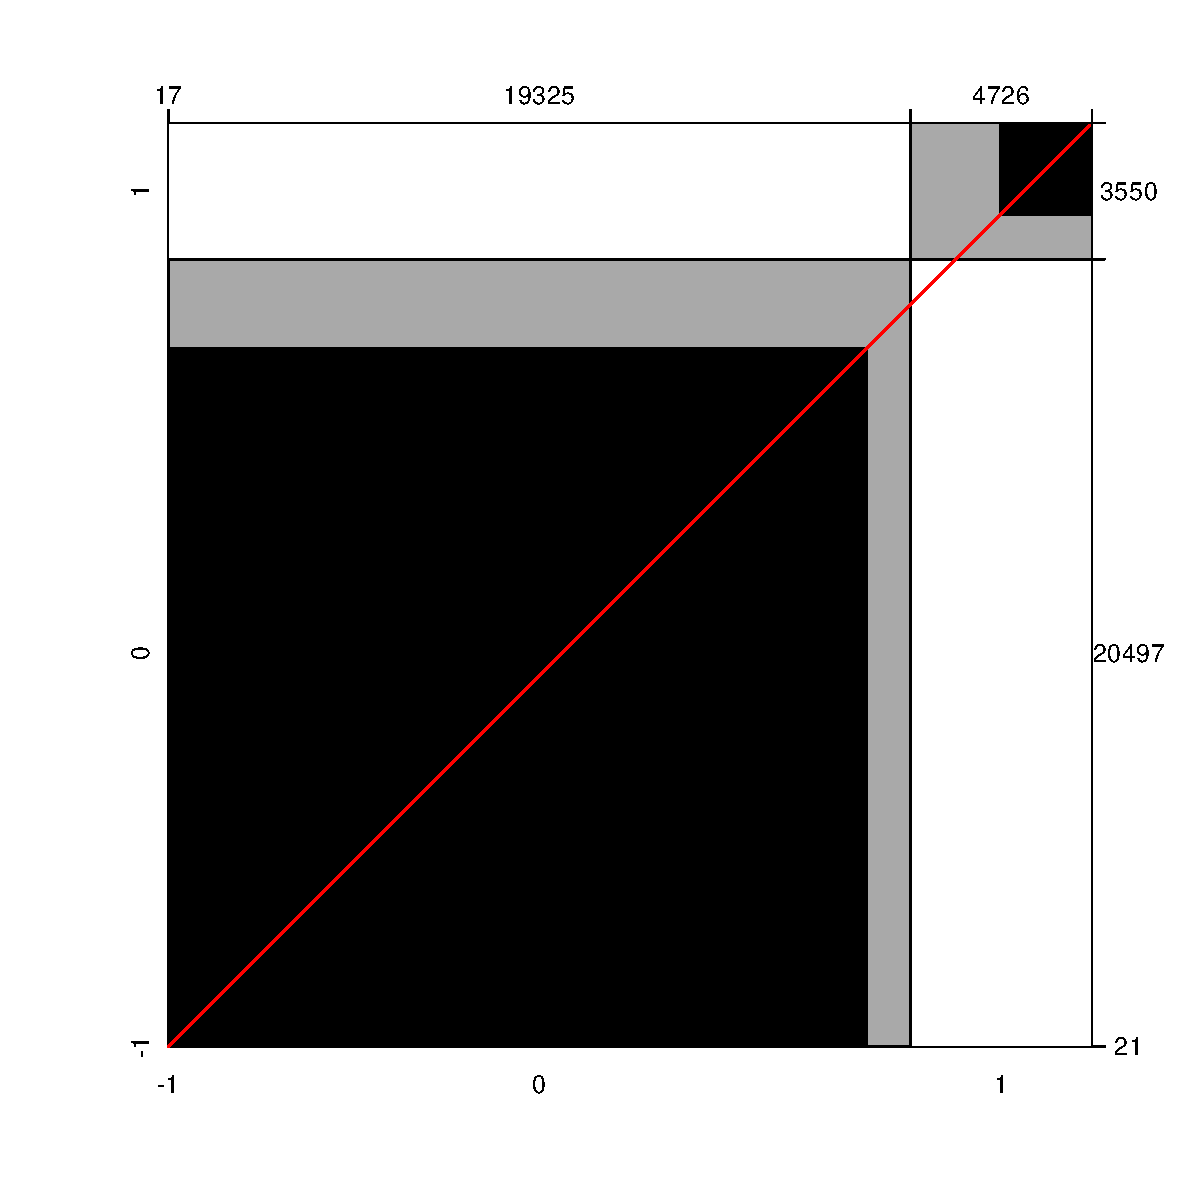
\includegraphics{supplementary_files/figure-latex/agreeplot-1.pdf}
\caption{\label{fig:agreeplot}Agreement plot showing the proportions of agreement between the two independent coders (ADL and CH). The dark spaces represent the proportion of agreement for the presence and absence of all aggregated variables in the entire dataset, and the gray spaces represent the proportions of disagreement for presence and absence.}
\end{figure}

\hypertarget{supplementary-results-in-study-1}{%
\section{Supplementary results in Study 1}\label{supplementary-results-in-study-1}}

This section outlines additional exploratory results from the cross-cultural study, based on data from the eHRAF and, in a few specified cases, from the SCCS.

\hypertarget{sccs-variables-used-for-the-pca}{%
\subsection{SCCS variables used for the PCA}\label{sccs-variables-used-for-the-pca}}

The SCCS consists of 186 cultures (rows) and 1781 culture-level variables (columns). As we describe in the main text, we filtered out these 1781 variables to include only those that are both quantitative measures (i.e., either ordinal or continuous variables) and complete, with no missing data for any of the 186 cultures. This resulted in 44 variables, which are listed in table S2.

\begin{table}

\caption{\label{tab:sccsvartable}Quantitative variables from the SCCS with no missing data that were used for our culture-level PCA.}
\centering
\fontsize{9}{11}\selectfont
\begin{tabular}[t]{l}
\toprule
SCCS variables\\
\midrule
Scale 1- Writing and Records\\
Scale 2- Fixity of Residence\\
Scale 3- Agriculture\\
Scale 4- Urbanization\\
Scale 5- Technological Specialization\\
\addlinespace
Scale 6- Land Transport\\
Scale 7- Money\\
Scale 8- Density of Population\\
Scale 9- Political Integration\\
Scale 10- Social Stratification\\
\addlinespace
Subsistence economy: gathering [Note, identical to EA001]\\
Subsistence economy: hunting [Note, identical to EA002]\\
Subsistence economy: fishing [Note, identical to EA003]\\
Subsistence economy: animal husbandry [Note, identical to EA004]\\
Subsistence economy: agriculture [Note, identical to EA005]\\
\addlinespace
Jurisdictional hierarchy of local community [Note, identical to EA032]\\
Date of publication\\
Number of pages in the book\\
Number of pages related to child training practices\\
Proportion of book devoted to child training\\
\addlinespace
Percent Importance of Agriculture in Contribution to Subsistence and Trade\\
Percent Importance of Domestic Animals in Contribution to Subsistence and Trade\\
Percent Importance of Fishing in Contribution to Subsistence and Trade\\
Percent Importance of Hunting in Contribution to Subsistence and Trade\\
Percent Importance of Gathering in Contribution to Subsistence and Trade\\
\addlinespace
Percent Importance of Trade in Contribution to Subsistence [and Trade]\\
Adequacy of HRAF File (in 1969)\\
Large Scale Slaveholding Systems: Recency\\
Large Scale Slaveholding Systems: Proportion of Slaves\\
Population Density (from Pryor Data)\\
\addlinespace
Population Density Data Quality: Inferences\\
Evil Eye Scaled Rating:\\
Evil Eye Belief\\
Pathogen stress: Leishmanias\\
Pathogen stress: Trypanosomes\\
\addlinespace
Pathogen stress: Malaria\\
Pathogen stress: Schistosomes\\
Pathogen stress: Filariae\\
Pathogen stress: Spirochetes\\
Pathogen stress: Leprosy\\
\addlinespace
Pathogen stress: Total Pathogen Stress\\
Frequency of External Warfare (Resolved Rating)\\
Pacification\\
Latitude\\
\bottomrule
\end{tabular}
\end{table}

\hypertarget{generalized-linear-mixed-models-based-on-cross-cultural-data}{%
\subsection{Generalized linear mixed models based on cross-cultural data}\label{generalized-linear-mixed-models-based-on-cross-cultural-data}}

We use a generalized logistic mixed model (GLMM) to model our PCA results (PC1: culture complexity and scale; PC2: pathogen stress, proximity to equator, and lower reliance on market economies) as predictors of presence/absence of supernatural theories of disease in the text records, with cultures as random intercepts. We found a ``statistically significant'' result, in which PC2 was positively associated with supernatural theories of disease, and PC1 was not clearly associated with the supernatural. See table S3.

\begin{table}[!htbp] \centering 
  \caption{Generalized logistic mixed model results for supernatural theories of disease predicted by the first two principal components from a cross-cultural PCA of the SCCS data. Estimates are log odds, with standard error in parentheses.} 
  \label{} 
\begin{tabular}{@{\extracolsep{5pt}}lc} 
\\[-1.8ex] & \multicolumn{1}{c}{\textit{Dependent variable:}} \\ 
\cline{2-2} 
\\[-1.8ex] & supernatural \\ 
\hline \\[-1.8ex] 
 pc1 & $-$0.03 \\ 
  & (0.04) \\ 
  & p = 0.53 \\ 
  & \\ 
 pc2 & 0.27 \\ 
  & (0.08) \\ 
  & p = 0.0003$^{***}$ \\ 
  & \\ 
 Constant & 1.11 \\ 
  & (0.14) \\ 
  & p = 0.00$^{***}$ \\ 
  & \\ 
\hline \\[-1.8ex] 
\textit{Note:}  & \multicolumn{1}{r}{$^{*}$p$<$0.05; $^{**}$p$<$0.01; $^{***}$p$<$0.001} \\ 
\end{tabular} 
\end{table}

This result, though interesting, should be viewed with skepticism. PC1 consists of cultural complexity variables, such as urbanization, population size and density, and cash- and market-based economies. PC2 consists of three underlying types of variables: Pathogen stress, proximity to the equator (absolute value of the latitude), and a low reliance on cash and market economies. An explanation that might \emph{seem} compelling, and is consistent with our hypotheses in the paper, is that pathogen stress is a key driver of supernatural theories of disease.

As we state in the main text, however, we can not draw this conclusion based on the association between PC2 and the supernatural, because pathogen stress is confounded by other contributing factors to PC2, such as latitude and cultural complexity. In fact, PC1 and PC2 are sufficiently related that we cannot even draw a firm conclusion about the apparent lack of effect of PC1 on the supernatural.

To see this, notice in table S4 that if pathogen stress is the sole predictor of supernatural, then as we might have expected, we find the weak positive association between pathogen stress and supernatural theories of disease. Adding latitude as a predictor, however, makes the effect of pathogen stress disappear. This is perhaps unsurprising; pathogen stress might be higher in tropical climates than in temperate ones. And yet, further complicating matters, adding PC1 (cultural complexity and scale) thereafter makes PC1 appear to have a significant negative effect on supernatural theories. See table S4.

\begin{table}[!htbp] \centering 
  \caption{Generalized logistic mixed model results for supernatural theories of disease predicted by the first two principal components from a cross-cultural PCA of the SCCS data. Estimates are log odds, with standard error in parentheses.} 
  \label{} 
\begin{tabular}{@{\extracolsep{5pt}}lccc} 
\\[-1.8ex] & \multicolumn{3}{c}{\textit{Dependent variable:}} \\ 
\cline{2-4} 
\\[-1.8ex] & \multicolumn{3}{c}{supernatural} \\ 
\hline \\[-1.8ex] 
 scale(pathogen\_stress) & 0.24 & $-$0.01 & 0.20 \\ 
  & (0.14) & (0.23) & (0.24) \\ 
  & p = 0.10 & p = 0.99 & p = 0.42 \\ 
  & & & \\ 
 scale(latitude) &  & $-$0.29 & $-$0.37 \\ 
  &  & (0.22) & (0.22) \\ 
  &  & p = 0.19 & p = 0.10 \\ 
  & & & \\ 
 scale(pc1) &  &  & $-$0.37 \\ 
  &  &  & (0.18) \\ 
  &  &  & p = 0.05$^{*}$ \\ 
  & & & \\ 
 Constant & 1.06 & 1.07 & 1.08 \\ 
  & (0.15) & (0.15) & (0.13) \\ 
  & p = 0.00$^{***}$ & p = 0.00$^{***}$ & p = 0.00$^{***}$ \\ 
  & & & \\ 
\hline \\[-1.8ex] 
\textit{Note:}  & \multicolumn{3}{r}{$^{*}$p$<$0.05; $^{**}$p$<$0.01; $^{***}$p$<$0.001} \\ 
\end{tabular} 
\end{table}

This is not to suggest that our analyses of PC1, PC2, and supernatural theories of disease is completely uninformative (quite the contrary). However, it does suggest that, as we conclude in the main text, confirmatory research is needed to directly test the hypothesis that pathogen stress is associated with supernatural theories of disease.

\newpage

\hypertarget{supplementary-results-in-study-2-maasai-field-data}{%
\section{Supplementary results in Study 2: Maasai field data}\label{supplementary-results-in-study-2-maasai-field-data}}

This section outlines additional data and results from the Maasai fieldwork study.

\hypertarget{participant-examples-of-conflict-between-science-and-religion}{%
\subsection{Participant examples of conflict between science and religion}\label{participant-examples-of-conflict-between-science-and-religion}}

When we asked participants about their views on science and religion, we specifically asked:

\begin{quote}
Sometimes people might have ideas that our beliefs about god make us disagree with. Do your beliefs about god ever make you disagree with the ideas that scientists, such as doctors, veterinarians, or agricultural specialists, might have?
\end{quote}

Some Maasai participants (\(N=12\)) agreed that scientific ideas sometimes conflict with their beliefs about god or religion. All of these participants were Christians. When asked as a follow-up question to give an example of how this might be the case, some (but not all) participants offered an example. The following quotations are examples of responses that were transcribed during interviews:

\begin{quote}
There may sometimes be ``satanic emotions'' in wise or educated people.
\end{quote}

\begin{quote}
For example, if doctors say that someone is HIV-positive then they will say that you have to take this medicine and that you might die. The person might start to worry that they will die and have fear because of what the doctor said to them. But the person who believes in god can pray, and it is the prayer, not the medicine, that will make them better.
\end{quote}

\begin{quote}
Sometimes scientists say there is no god, which I disagree with.
\end{quote}

\begin{quote}
Science says that there is no god, but we believe differently. The scientists and doctors will not be disturbed by this if they have faith in god also.
\end{quote}

\begin{quote}
Sometimes I disagree with scientists and teachers if they might say, for example, that there is no god.
\end{quote}

\begin{quote}
I will sometimes disagree with doctors or scientists if they do not think that god exists or if they are not Christians. But this does not happen if they separate those beliefs with their work.
\end{quote}

\begin{quote}
My beliefs in god sometimes make me disagree with scientists; unbelievable things in the world are not man-made, but are made by god. Doctors do good things by treating other people though.
\end{quote}

\hypertarget{mosaic-plot-of-preferred-specialists-for-serious-illnesses}{%
\subsection{Mosaic plot of preferred specialists for serious illnesses}\label{mosaic-plot-of-preferred-specialists-for-serious-illnesses}}

As we show in the main text, participants overwhelmingly preferred to use the clinic in cases of serious illness, though many also preferred to use either friends, family, or religious specialists. We reported these preferences in the main text by religious identity. Here, we include them in the aggregate to show how strongly the clinic was preferred overall, and how religious options (the church and the laibon) both slightly increased after the first option would hypothetically fail. The clinic was the most popular first option, but as seen in the main text, some participants defaulted initially to family and friends as their first option, but fell back on the clinic as their second option. See figure \ref{fig:fieldplotillness}.

\begin{figure}[p]

{\centering 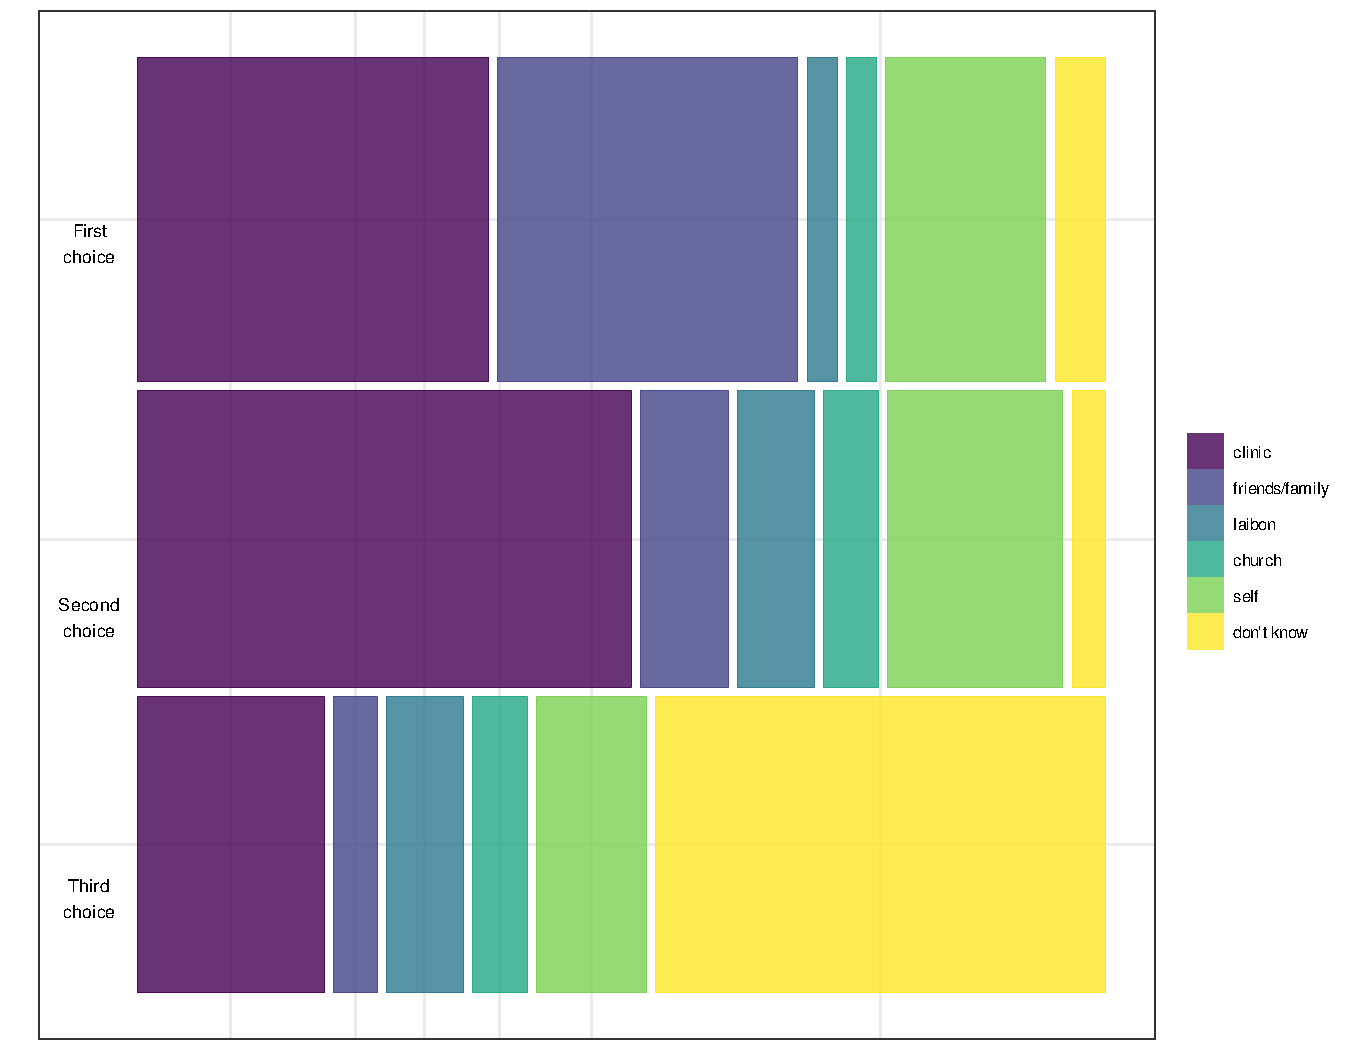
\includegraphics{supplementary_files/figure-latex/fieldplotillness-1} 

}

\caption{Mosaic plot of the proportions of participants who identified different types of specialists as their first, second, and third choices to help them in the case of having a serious illness. Colors represent categories of responses given by participants in each option.}\label{fig:fieldplotillness}
\end{figure}

\hypertarget{pca-results-for-explanations-of-how-herbal-medicines-work}{%
\subsection{PCA results for explanations of how herbal medicines work}\label{pca-results-for-explanations-of-how-herbal-medicines-work}}

After coding for presence/absence of content features of each participant's explanation of how a common herbal medicine works, we concluded based on visual inspection of the heatmap (figure 14 in the main text) that people were broadly divided into ``don't know'', ``knowing when/how to make the medicine'', and and ``mechanistic'' explanations that use substance and essence terms. We also conducted a PCA on the binary data matrix of these responses. PC1 showed that participants who did not know how the medicine worked, and/or did not have a working model of the mechanisms by which the medicine worked, tended to be associated with explanations invoking the conditions under which a person should prepare the medicine, whereas explanations tended to invoke substances, essences, and physiological terms. See figure \ref{fig:pcaExplain}.

\begin{figure}[p]

{\centering 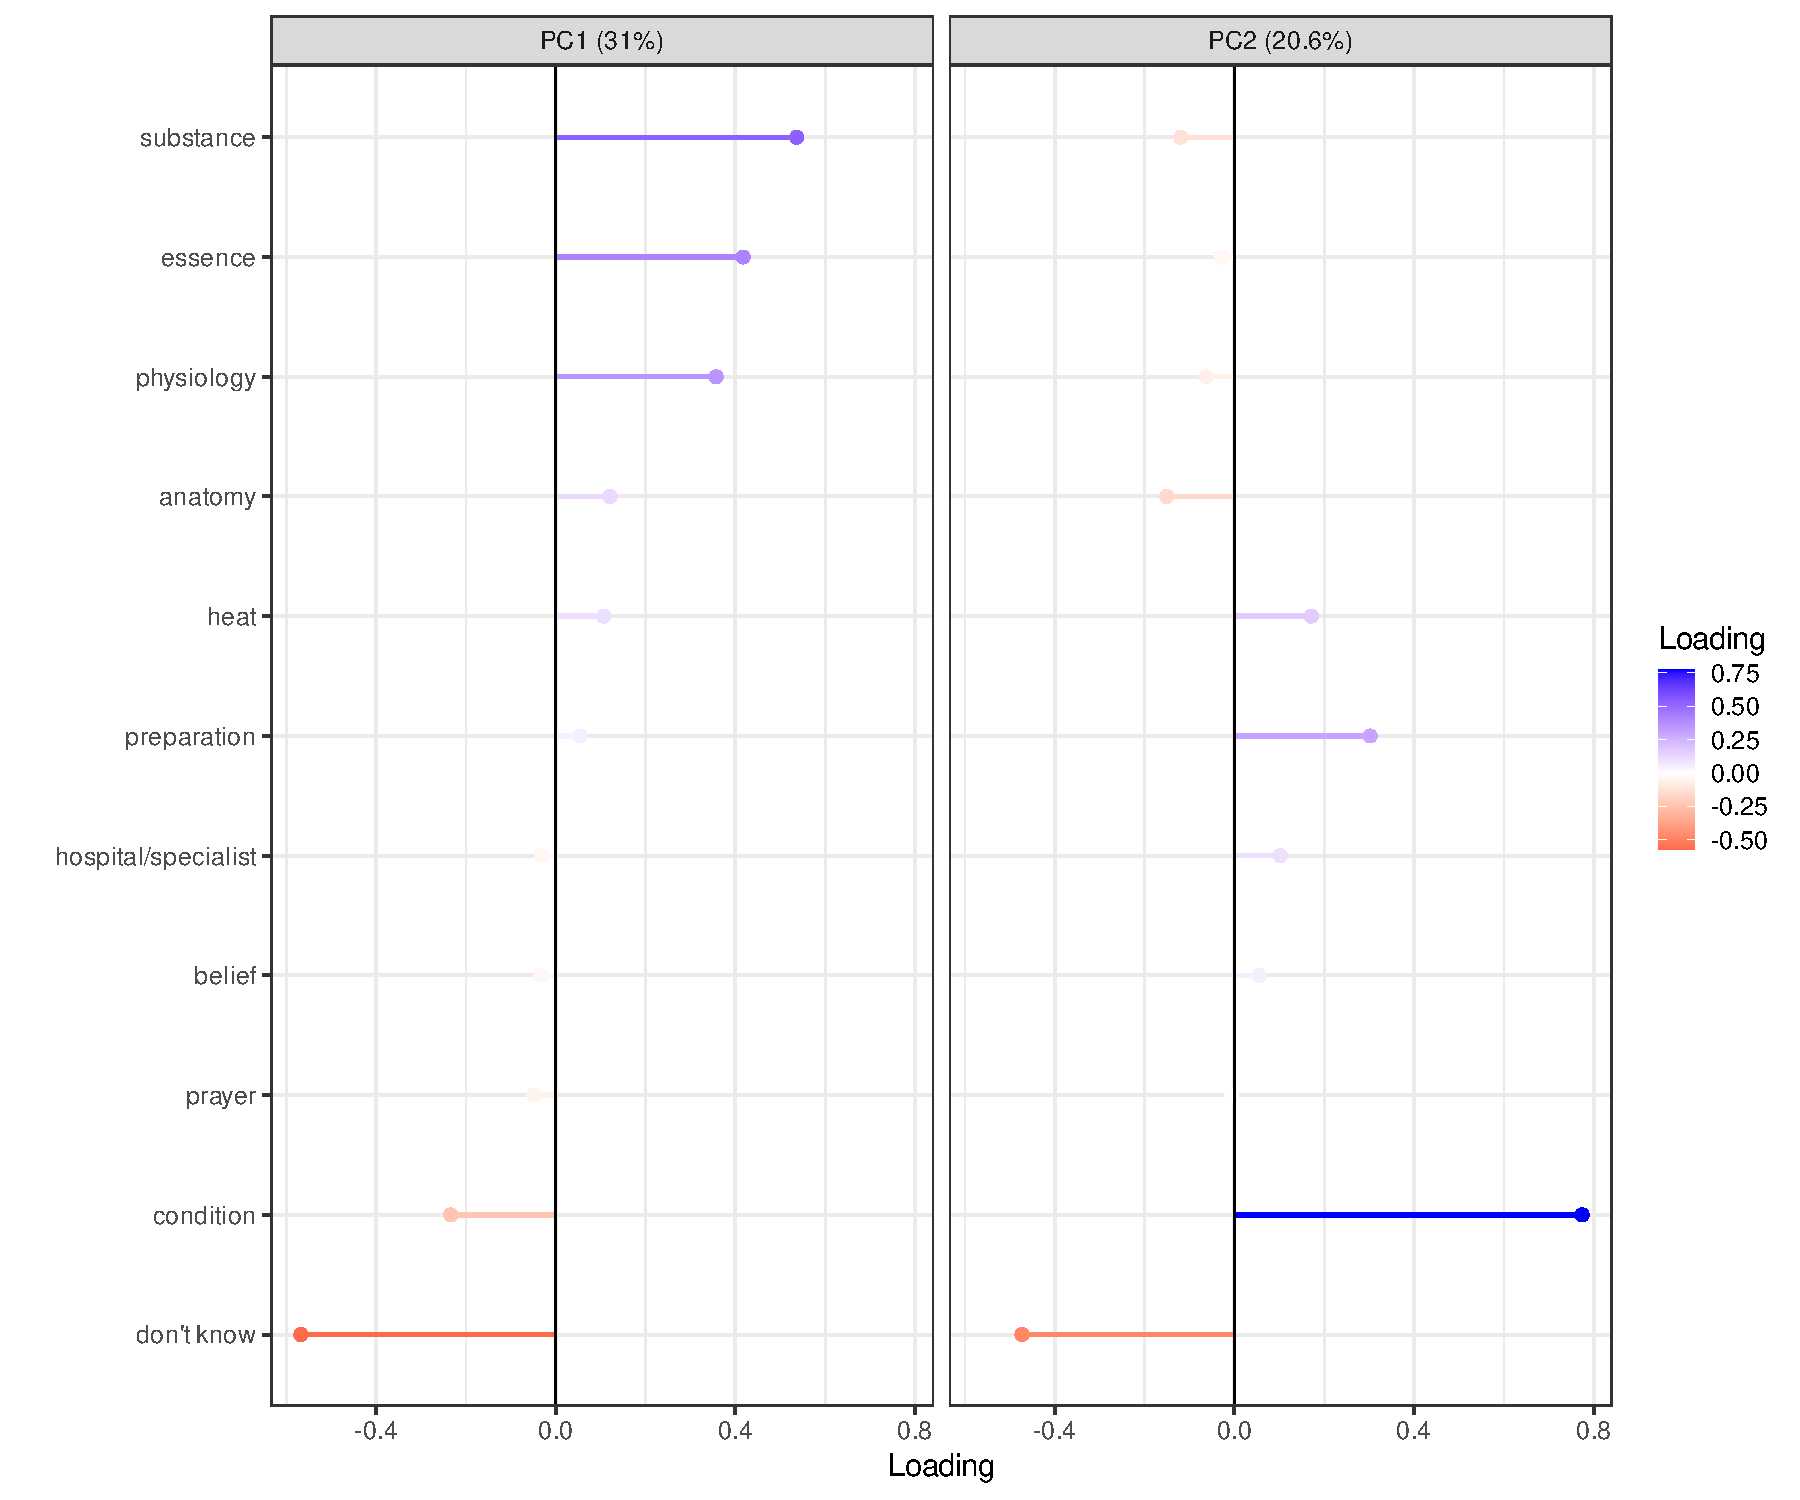
\includegraphics{supplementary_files/figure-latex/pcaExplain-1} 

}

\caption{PCA loadings on the first two principal components in the explanations of how herbal medicine works among Maasai participants. PC1 corresponds to knowledgeability and detail of explanation, and PC2 corresponds to the necessary conditions and preparation steps for making the medicine.}\label{fig:pcaExplain}
\end{figure}

\end{document}
